\documentclass{article}
\usepackage[utf8]{inputenc}
\usepackage{natbib}
\usepackage[T1]{fontenc}
\usepackage[francais]{babel}
\usepackage{chemist}
\usepackage{array}
\usepackage[version=3]{mhchem}
\usepackage{amsmath}
\usepackage[squaren,Gray]{SIunits}
\usepackage{numprint}
\usepackage{amsfonts}
\usepackage{amssymb}
\usepackage{graphicx}
\usepackage{mathtools}
\usepackage{fullpage}
\usepackage{mhchem}
\usepackage{listings}
\usepackage{hyperref}
\usepackage{mathenv} %%%%%%%%%%% do not forget to add to head.tex
\usepackage{empheq} %%%%%%%%%%%% same
\author{Groupe 1246 }


\title{\vspace{\fill}\begin{LARGE} \begin{bf}  
Rapport de la première tâche: deuxième version \\
LFSAB1503 \\ 
\end{bf}\end{LARGE}
\vspace{\fill}}
\begin{document}
\maketitle
\newpage
\tableofcontents
\newpage
\newpage
\section{Introduction}

Ce premier document est une pré-étude au sujet de la production d'ammoniac à partir de méthane. 
Il comprend les bilans de matière et d'énergie du procédé, ainsi qu'un flowsheet simplifié. L'analyse paramétrique 
présentée est basée sur un programme \textsc{Matlab} permettant de déterminer les quantités de réactifs nécessaires
à la production d'une certaine quantité d'ammoniac. Notons que ce programme se basait sur beaucoup d'hypothèses 
simplificatrices; il n'était donc pas optimal lors de la rédaction de cette première tâche. La version disponible en annexe
est une forme améliorée.
Les deux paramètres que nous pouvions faire varier étaient:

\begin{enumerate}
\item la température de sortie du réacteur de reformage à la vapeur de méthane.
\item la quantité d'ammoniac \ce{NH_3} produite par jour.
\end{enumerate}


Nous entamerons ce document par le bilan de matière, pour continuer avec le bilan d'énergie. Nous détaillerons ensuite le nombre de tuyaux
dans le réacteur primaire de reformage, et poursuivrons par l'analyse paramétrique. 

\newpage

%laissez sans \usepackage et \begin svp
\section{Bilan de matière}

\subsection{Introduction et notations}

Cette section met en avant l'évolution des réactifs et produits en terme de débit. 
Nous pouvons ainsi gérer les quantités de matière nécessaires à la réaction par unité de temps, et
moduler la production d'ammoniac. Nous avons procédé de manière systématique, en partant de la première
équation jusqu'à la dernière, et en posant quelques 
variables intermédiaires:

\begin{itemize}
	\item Soit $x$ le nombre de moles de \ce{CH4} introduites dans le réacteur par jour.
	\item Soit $y$ le nombre de moles d'\ce{H2O} introduites dans le réacteur par jour.
	\item Soit $m$ le degré d'avancement de la réaction à l'équilibre 1.
	\item Soit $n$ le degré d'avancement de la réaction à l'équilibre 2.
	\item Soit $a$ le nombre de moles d'air introduites dans le réacteur par jour.
\end{itemize}

\subsection{Analyse et commentaires}
Dans la phase de reformage primaire, les réactions sont à l'équilibres; ce qui signifie qu'il faudra prendre en 
compte un degré d'avancement lié à la température par la constante d'équilibre. Pour le moment, nous ne devons pas 
nous en préoccuper, et nous poserons seulement les variables $m$ et $n$ identifiées ci-dessus. 

\begin{figure}[h]
\begin{center}
\begin{tabular}{|c|c|c|c|c|}
\hline
&
\multicolumn{1}{c!{\makebox[0pt]{+}}}{
\ce{CH4}}
&
\multicolumn{1}{c!{\makebox[0pt]{$\rightleftharpoons$}}}{\ce{H2O}}
&
\multicolumn{1}{c!{\makebox[0pt]{+}}}{\ce{3H2}}
& \ce{CO}
\\
\hline
$n_i$ & $x$ & $y$ & $0$ & $0$ \\
\hline
$n_f$ & $x-m$ & $y-m-n$ & $3m+n$ & $m-n$ \\\hline
\end{tabular}
\end{center}
\caption{Tableau d'avancement de la réaction 1 du reformage primaire.}
\end{figure}
\begin{figure}[h]
\begin{center}
\begin{tabular}{|c|c|c|c|c|}
\hline
&
\multicolumn{1}{c!{\makebox[0pt]{+}}}{
\ce{CO}}
&
\multicolumn{1}{c!{\makebox[0pt]{$\rightleftharpoons$}}}{\ce{H2O}}
&
\multicolumn{1}{c!{\makebox[0pt]{+}}}{\ce{H2}}
& \ce{CO2}
\\
\hline
$n_i$ & $m$ & $y-m$ & $3m$ & $0$\\
\hline
$n_f$ & $m-n$ & $y-m-n$ & $3m+n$ & $n$ \\\hline
\end{tabular}
\end{center}
\caption{Tableau d'avancement de la réaction 2  du reformage primaire.}
\end{figure}

Les réactions suivantes sont toutes considérées comme complètes. Dans le reformeur secondaire, le méthane et l'oxygène
sont alimentés de façon stœchiométrique, ce qui signifie qu'il ne reste plus aucun de ces deux réactifs après réaction.
Tout a été converti. Cette condition nous permet d'aboutir à une première équation :
$$x - m - 2\cdot0.21a = 0$$

\begin{figure}[h]
\begin{center}
\begin{tabular}{|c|c|c|c|c|}
\hline
&
\multicolumn{1}{c!{\makebox[0pt]{+}}}{
\ce{2CH4}}
&
\multicolumn{1}{c!{\makebox[0pt]{$\rightarrow$}}}{\ce{O2}}
&
\multicolumn{1}{c!{\makebox[0pt]{+}}}{\ce{2CO}}
& \ce{4H2}
\\
\hline
$n_i$ & $x-m$ & $0.21a$ & $m-n$ & $3m+n$\\
\hline
$n_f$ & $0$ & $0$ & $x-n$ & $m+n+2x$ \\\hline
\end{tabular}
\end{center}
\caption{Tableau d'avancement de la réaction du reformage secondaire}
\end{figure}

Dans le réacteur Water-Gas-Shift, tout le \ce{CO} aura réagi, mais il faudra séparer
l'eau restante, et absorber le \ce{CO2}. Nous obtenons l'expression du nombre de moles d'eau sortant grâce au tableau .

\begin{figure}[h]
\begin{center}
\begin{tabular}{|c|c|c|c|c|}
\hline
&
\multicolumn{1}{c!{\makebox[0pt]{+}}}{
\ce{CO}}
&
\multicolumn{1}{c!{\makebox[0pt]{$\rightarrow$}}}{\ce{H2O}}
&
\multicolumn{1}{c!{\makebox[0pt]{+}}}{\ce{H2}}
& \ce{CO2}
\\
\hline
$n_i$ & $x-n$ & $y-m-n$ & $m+n+2x$ & $n$\\
\hline
$n_f$ & $0$ & $y-m-x$ & $m+3x$ & $x$ \\\hline
\end{tabular}
\end{center}
\caption{Tableau d'avancement de la réaction dans les réacteurs Water-Gas-Shift.}
\end{figure}

Enfin, la dernière réaction permet la synthèse de \ce{NH3}. Nous imposons qu'il
ne reste ni de \ce{N2} ni de \ce{H2}, étant donné que la réaction globale peut être considérée
comme complète, grâce au "recyclage".
Nous obtenons ici une seconde équation:
$$ 2\cdot0.78a = \frac{2}{3}\cdot (m + 3x) $$

\begin{figure}[h]
\begin{center}
\begin{tabular}{|c|c|c|c|}
\hline
&
\multicolumn{1}{c!{\makebox[0pt]{+}}}{
\ce{N2}}
&
\multicolumn{1}{c!{\makebox[0pt]{$\rightarrow$}}}{\ce{3H2}}
&
\ce{2NH3}
\\
\hline
$n_i$ & $0.78a$ & $m+3x$ & $0$ \\
\hline
$n_f$ & $0$ & $0$ & $2\cdot0.78 a$ \\\hline
\end{tabular}
\end{center}
\caption{Tableau d'avancement de la synthèse de l'ammoniac}
\end{figure}

Au terme de ce procédé, nous aurons donc produit $1.56a$ moles de \ce{NH3}. Cette quantité est liée au
nombre de moles de \ce{CH4} introduites dans le réacteur (i.e. $x$) par les deux équations obtenues plus haut:
\[
\left \{
\begin{array}
& x - m - 2\cdot0.21a = 0
& 2\cdot0.78a = \frac{2}{3}\cdot (m + 3x) 
\end{array}
\right.
\]
En simplifiant, on obtient: $4x = 2.76\cdot a$. Nous avons maintenant la quantité de \ce{CH4} introduite
dans le réacteur par jour en fonction de la quantité d'ammoniac produite. Notons que la température n'a pas d'effet
sur cette quantité. Mais nous n'avons pas encore d'information à propos de la quantité d'eau nécessaire.


Afin d'obtenir une relation avec le nombre de moles d'\ce{H2O} introduites dans le réacteur (i.e. $y$), nous
devons utiliser les constantes d'équilibre des deux premières réactions. Pour une certaine
température $T$ [\unit{}{\kelvin}], nous avons l'expression suivante pour $K_1 (T)$ et $K_2 (T)$ , respectivement les
constantes d'équilibre de la première et de la deuxième équation:
\[
\left \{
\begin{array}
& K_1 (T) = \left( \dfrac{(3m+n)^3 \cdot (m-n) \cdot p_{tot}^3}{(x+2m+y)^2 \cdot (y-m-n) \cdot (x-m) \cdot p_0^2}\right)
& K_2 (T) = \left( \dfrac{(3m+n)\cdot n}{(m-n)\cdot(y-m-n)} \right)
\end{array}
\right.
\]
Nous pouvons calculer la valeur théorique de ces constantes d'équilibre en fonction de la température
avec \textsc{Matlab} (voir code en Annexe), en posant la pression du reformeur primaire à \unit{30}{\bbar}\footnote{Valeur conseillée sur iCampus}.
Il nous reste donc \numprint{4} équations à \numprint{4} inconnues et \numprint{2} paramètres: la
température $T$ et $a$ le nombre de moles d'air introduites dans le réacteur. À partir de ces équations, nous avons
créé un outil de gestion permettant de réaliser le calcul d'approvisionnement nécessaire en matière première, en
fonction de la température et de la capacité d'ammoniac à produire. Le code est disponible en Annexe.%prog final matlab complet


\newpage

\section{Bilan d'énergie}

Cette section traite le bilan énergétique du procédé étudié.
Sur base du flow-sheet simplifié disponible ci-après, nous avons déterminé que seulement trois réactions
devaient être analysées pour réaliser un tel bilan: celle se produisant dans le bloc du four et celles dans 
le réacteur du reformage primaire. Grâce à cette analyse, nous obtiendrons une expression pour la quantité de \ce{CH4} nécessaire pour la production d'une certaine quantité d'ammoniac, à une certaine température.

\subsection{Le bloc "Réacteur de reformage primaire"}

Dans ce bloc, nous devons traiter les deux réactions à l'équilibre suivantes, prenant place simultanément, à une certaine température $T$:

\begin{equation}\label{eq:Reaction1}
\ce{CH_{4(g)} + H_{2}O_{(g)} <=> 3H_{2(g)} + CO_{(g)}}
\end{equation}
\begin{equation}\label{eq:Reaction2} {\ce{CO_{(g)} + H_{2}O_{(g)} <=>  H_{2(g)} + CO_{2(g)}}}
\end{equation}


\bigbreak
Nous allons développer le raisonnement que nous avons effectué afin d'obtenir l'expression de la différence d'enthalpie dans le réacteur et, dans un premier temps, nous ne nous intéresserons qu'à la première des deux réactions. Fondamentalement, nous savons que:
$$\Delta H\degree_{Reaction1}(T)=3\Delta H\degree_{H_{2(g)}}(T) + \Delta H\degree_{CO_{(g)}}(T) -
\lbrack\Delta H\degree_{CH_{4(g)}}(T) + \Delta H\degree_{H_{2}O_{(g)}}(T)\rbrack$$

Pour rappel, l'enthalpie standard d'une espèce chimique à une certaine température $T$ s'écrit: \begin{equation}\label{eq:deltaH}
\Delta H\degree(T)=\Delta H\degree(T_{ref})  + \displaystyle \int_{T_{ref}}^{T} C_{p}(T) \mathrm{d}T
\end{equation}


Les enthalpies à une température de référence (typiquement, $T_{ref}=\unit{25}{\celsius}=\unit{298}{\kelvin}$) sont disponibles dans des tables de mesures expérimentales. Il ne nous reste donc plus qu'à trouver l'expression de $C_p$, la capacité thermique à pression constante, en fonction de $T$.
Après quelques recherches\cite{NIST}, nous avons trouvé la formule suivante: \begin{equation}\label{eqref:capacite}
C_p=A+\dfrac{BT}{1000}+C\left(\dfrac{T}{1000}\right)^2+D\left(\dfrac{T}{1000}\right)^3+E\left(\dfrac{1000}{T}\right)^2
\end{equation} où $A,B,C,D,E$ sont des constantes propres à chaque composant (cfr. Annexe).
En remplaçant, nous pouvons facilement obtenir une expression pour $\Delta H\degree_{Reaction1}$, que nous ne retranscrirons pas
ici, mais qui est disponible dans le code \textsc{MATLAB} en Annexe. 
Les calculs pour la deuxième réaction à l'équilibre étant similaires, nous pouvons
calculer $\Delta H\degree_{Reaction2}(T)$ sans difficulté. A fin de calculer la différence d'enthalpie dans le réacteur
il nous faut connaître les degrés d'avancement des réactions calculées dans le bilan de matière. Ainsi, nous trouvons la relation suivante, où $m$ et $n$ sont respecitvement les degrés d'avancement de la réaction (\ref{eq:Reaction1}) et de la réaction (\ref{eq:Reaction2}):
\begin{equation}\label{eq:deltaHreacteur}\Delta H\degree_{Reacteur}(T)=m\cdot\Delta H\degree_{Reaction1}(T)+n\cdot\Delta H\degree_{Reaction2}(T)}\end{equation}

\subsection{Le bloc "Four"}
La réaction ayant lieu dans le four n'est autre que la combustion du méthane:

\begin{equation}\label{combust.methane}\ce{CH_{4(g)} + 2O_{2(g)} <=> 2H_2O_{(g)} + CO_{2(g)}}\end{equation}

De plus, nous savons que:

$$\Delta H\degree_{Four} = 2\cdot \Delta H\degree_{H_{2}O_{(g)}} + \Delta H\degree_{CO_{2(g)}}
- \left(\Delta H\degree_{CH_{4(g)}} + 2\cdot \Delta H\degree_{O_{2(g)}}\right)$$

Nous considèrerons que la réaction du four se passe également à la température $T$. 
Nous devons donc à nouveau trouver la valeur du $\Delta H\degree(T)$ de chaque composé grâce à la formule (\ref{eq:deltaH}),
puis injecter ces valeurs dans l'équation du $\Delta H\degree_{Four}$ -- ces calculs, vu leur longueur, ne sont pas repris dans
ce document. Nous supposons que la réaction à la température $T$ sera exothermique car le four sert à fournir de l'énergie à la réaction
endothermique du réacteur primaire de reformage. 
Nous sommes maintenant en mesure d'exprimer $DB$, la quantité de \ce{CH_4} nécessaire dans le four:

$DB = \dfrac{\Delta H_{Reacteur}}{\Delta H_{Four} }\unit{}{\mole\per jour}$


\newpage

\section{Nombre de tuyaux dans le réacteur primaire de reformage}
Dans cette section, nous allons déterminer le nombre de tuyaux de diamètre valant $d=\unit{10}{\centi\meter}$ que doit comporter 
le réacteur de reformage. On considère que la vitesse superficielle typique à l'entrée du réacteur est de 
\unit{2}{\meter\per\second}. Le résultat que nous allons obtenir dépendra de deux paramètres: la température du réacteur,
et la quantité d'ammoniac produite. Nous introduisons la notation $\dot{V}$ pour désigner le débit volumique (exprimé
en unités de volume par unité de temps). En supposant que les gaz sont parfaits, nous pouvons exprimer le flux
de $\ce{CH_4}$ et d'$\ce{H_2O}$, grâce à la relation $p\cdot F_{vol}=F_{mol}\cdot R\cdot T$ où $F_{mol}$ est le flux
molaire et $F_{vol}$ le flux volumique. Les deux composés se déplaçant simultanément dans les tuyaux, le nombre de tuyaux $N$ se trouve via la relation suivante:

$$N = \dfrac{F_{mol,\ce{CH_4}} + {F_{mol,\ce{H_2O}}}}{F_{vol}}$$

Grâce à notre outil de calcul de bilan de matière (en Annexes), dans le cadre d'une production journalière de 
\unit{1500}{t} d'ammoniac à \unit{1080}{\kelvin}, nous pouvons déterminer le nombre de tuyaux nécessaires:

$$N = (F_{mol,\ce{CH_4}}+F_{mol,\ce{H_2O}}) \cdot \dfrac{R \cdot T}{p \cdot F_{vol}} = (3.8956\cdot 10^7+7.6798\cdot 10^7}}) \cdot \dfrac{8.31451 \cdot 1080}{30\cdot 10^5 \cdot(0.05^2\pi\cdot2\cdot3600\cdot24)}} = 233$$

Le résultat est donc \numprint{233} tuyaux.

\newpage
\section{Analyse paramétrique}
\paragraph{} Après avoir conçu l'outil de gestion du plant, il est intéressant d'analyser les résultats obtenus en
faisant varier les paramètres dans une plage réaliste. Les tableaux ci-dessous reprennent cette analyse. Nous avons
considéré une variation de température de \unit{800}{\kelvin} à \unit{1300}{\kelvin}. Ce choix a été déterminé par
les valeurs de référence utilisées dans le calcul de $K(T)$, qui sont pour la plupart valables jusqu'à
\unit{1300}{\kelvin}. En ce qui concerne la quantité d'ammoniac produite, nous avons testé de \unit{1000}{\ton \per jour} à
\unit{2000}{\ton \per jour}, étant donné que c'est la capacité typique d'un plant d'ammoniac.

\paragraph{} Le premier tableau fait varier la température, en considérant la quantité d'ammoniac \ce{NH_3} produite
par jour constante et valant \unit{1500}{\ton \per jour}.
\begin{table}[h!]
\centering
\begin{tabular}{|c||c|c|c|}
\hline
Température & Débit de méthane \ce{CH_4} & Débit de l'eau \ce{H_{2}O} & Débit d'air \\
\unit{\kelvin} & [\unit{\meter^3\per jour}] & [\unit{\meter^3\per jour}] & [\unit{\meter^3\per jour}] \\
\hline
800 & 86373.59 & 1044242.84 & 1.2518e+05 \\
\hline
900 & 97170.29 & 491179.16 & 1.4083e+05 \\
\hline
1000 & 107966.99 & 234055.84 & 1.5647e+05 \\
\hline
1100 & 118763.69 & 105168.26 & 1.7212e+05 \\
\hline
1200 & 129560.39 & 62398.32 & 1.8777e+05 \\
\hline
1300 & 140357.09 & 57193.98 & 2.0342e+05 \\
\hline
\end{tabular}
\caption{La température $T$ varie, la quantité d'ammoniac \ce{NH_3} produite par jour est constante}
\label{tab:tvarie}
\end{table}
\paragraph{} Le deuxième tableau fait varier la quantité d'ammoniac \ce{NH_3}, en considérant la température $T$ constante et
valant \unit{1000}{\kelvin}.
\begin{table}[h!]
\centering
\begin{tabular}{|c||c|c|c|}
\hline
Production journalière de \ce{NH_3} & Débit de méthane \ce{CH_4} & Débit de l'eau \ce{H_{2}O} & Débit d'air \\
\unit{\ton \per jour} & [\unit{\meter^3\per jour}] & [\unit{\meter^3\per jour}] & [\unit{\meter^3\per jour}] \\
\hline
\hline
1000 & 71978.00 & 156037.22 & 1.0432e+05 \\
\hline
1100 & 79175.80 & 171640.95 & 1.1475e+05 \\
\hline
1200 & 86373.59 & 187244.67 & 1.2518e+05 \\
\hline
1300 & 93571.39 & 202848.39 & 1.3561e+05 \\
\hline
1400 & 100769.19 & 218452.11 & 1.4604e+05 \\
\hline
1500 & 107966.99 & 234055.84 & 1.5647e+05 \\
\hline
1600 & 115164.79 & 249659.56 & 1.6691e+05 \\
\hline
1700 & 122362.59 & 265263.28 & 1.7734e+05 \\
\hline
1800 & 129560.39 & 280867.00 & 1.8777e+05 \\
\hline
1900 & 136758.19 & 296470.73 & 1.9820e+05 \\
\hline
2000 & 143955.99 & 312074.45 & 2.0863e+05 \\
\hline
\end{tabular}
\caption{La quantité d'ammoniac \ce{NH_3} produite par jour varie, la température $T$ est constante}
\label{tab:nh3varie}
\end{table}

\newpage
Nous devions surtout surveiller la quantité d'eau, étant donné qu'elle devait être en excès dans les réactions à
l'équilibre, pour qu'il reste assez de vapeur afin de permettre une conversion complète de \ce{CO} en \ce{CO2} dans le
réacteur Water-Gas-Shift.
Nous avons donc déterminé la température critique à partir de laquelle la quantité d'eau sortante devenait nulle.
Nous sommes arrivés à la conclusion qu'il faut limiter la température de sortie du reformeur primaire à
\unit{1049.472}{\kelvin}, si nous voulons une capacité d'ammoniac de \unit{1500}{\ton\per jour}.
Le graphe suivant permet de visualiser ce qui sort vraiment de notre installation. Les valeurs ont été calculées pour
avoir 1500t d'ammoniac au final. Il est donc normal de constater que l'ammoniac apparaît en ligne droite.
Nous pouvons égalemnt bien visualiser qu'à partir de la température de \unit{1050}{\kelvin}, le débit d'eau sortant devient
négatif; chose problématique comme expliqué ci-dessus.
Le \ce{CO2} et l'argon sortant sont quant à eux constants en fonction de la température. L'argon est rejeté en petites quatités, mais le \ce{CO2}
apparaît en quantités plus importantes malheureusement.
\begin{figure}[ht!]
\centering
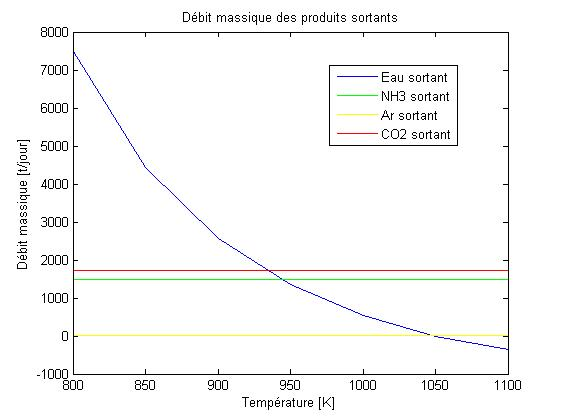
\includegraphics[scale=0.6]{produits.jpg}
\label{produits_sortants}
\end{figure}

\newpage
\section{Conclusion}
Le but de cette première tâche était de créer un outil de gestion régissant une production d'ammoniac. 
Pour cela, nous nous sommes basés sur un flow-sheet simplifié, à partir duquel nous avons établi le bilan d'énergie du processus
ainsi qu'un bilan de matière. Pour le bilan d'énergie nous nous sommes uniquement focalisés sur le bloc "reformage primaire" ainsi
que sur le bloc "four" comme expliqué dans la section bilan d'énergie. Par la suite, nous avons fait un bilan de matière 
afin d'exprimer les quantités de matière necessaires pour une production voulue d'ammoniac. Une fois ces deux bilan 
réalisés, nous avons conçu un outil de gestion grâce au programme \textsc{MATLAB}. L'outil de gestion permet de déterminer les 
quantités d'eau et de méthane nécessaires en fonction de deux variables, à savoir la capacité du plant et la température à 
la sortie du réacteur de reformage. En plus de cela, nous avons calculé le nombre de tuyaux nécessaires dans le réacteur
primaire de reformage pour une production journalière de $\unit{1500}{\tonne}$ à une température de sortie de 
$\unit{1080}{\kelvin}$.

\newpage
\section{Annexe}
\subsection{Donnees et constantes}
On connait les valeurs de $\Delta H\degree (\unit{25}{\celsius})$ pour les éléments suivants:

\begin{itemize}
\item{\ce{CH_{4(g)}} $\Rightarrow \unit{-74.6}{\kilo\joule\per\mole}$}
\item{\ce{H_2O_{(g)}} $\Rightarrow \unit{-241.83}{\kilo\joule\per\mole}$}
\item{\ce{CO_{(g)}} $\Rightarrow \unit{-110.53}{\kilo\joule\per\mole}$}
\item{\ce{CO_{2(g)}} $\Rightarrow \unit{-393.51}{\kilo\joule\per\mole}$}
\item{\ce{H_{2(g)}} $\Rightarrow \unit{0}{\kilo\joule\per\mole}$}
\item{\ce{O_{2(g)}} $\Rightarrow \unit{0}{\kilo\joule\per\mole}$}
\end{itemize}

On connaît les constantes permettant d'utiliser la formule (\ref{eqref:capacite}):

\begin{table}[h]
\centering
\begin{tabular}{|c|c|c|c|c|c|}
\hline 
\rule[-1ex]{0pt}{2.5ex}  & A & B & C & D & E \\ 
\hline 
\rule[-1ex]{0pt}{2.5ex} \ce{CH_{4(g)}} & -0.703 & 108.471 & -42.521 & 5.862 & 0.678 \\ 
\hline 
\rule[-1ex]{0pt}{2.5ex} \ce{H_2O_{(g)}} & 30.092 & 6.832 & 6.793 & -2.534 & 0.082 \\ 
\hline 
\rule[-1ex]{0pt}{2.5ex} \ce{CO_{(g)}} & 25.5675 & 6.0961 & 4.0546 & -2.6713 & 0.131 \\ 
\hline 
\rule[-1ex]{0pt}{2.5ex} \ce{CO_{2(g)}} & 34.2244 & 41.044 & -23.5297 & 5.5352 & -0.129 \\ 
\hline 
\rule[-1ex]{0pt}{2.5ex} \ce{H_{2(g)}} & 33.066 & -11.363 & 11.432 & -2.772 & -0.158 \\ 
\hline 
\end{tabular} 
\caption{Tableau des constantes pour la formule (\ref{eqref:capacite})}
\label{tab:my_label}
\end{table}

\subsection{Flowsheet du plant}

\begin{figure}[h]
   \includegraphics[scale=0.4]]{flowsh}
\end{figure}

\subsection{Code \textsc{MATLAB}}
Voici une fonction en \textsc{MATLAB} créée par nos soins, nous permettant de calculer l'enthalpie d'un élément à une certaine
température $T$, en fonction des différentes constantes utilisées dans la formule (\ref{eqref:capacite}).
\lstset{language=Matlab,breaklines=true}
\begin{lstlisting}[frame=single]
\lstinputlisting{T(K)matlab.m}
\end{lstlisting}



\nocite{*}
\bibliographystyle{plain} % Le style est mis entre accolades.
\bibliography{sources} % mon fichier de base de données s'appelle bibli.bib
\end{document}
